\documentclass[conference]{IEEEtran}
\IEEEoverridecommandlockouts

\usepackage{amsmath,amssymb}
\usepackage{graphicx}
\usepackage{booktabs}
\usepackage{multirow}
\usepackage{url}
\usepackage{cite}
\usepackage{xcolor}

\graphicspath{{figures/}}

\begin{document}

\title{Beyond the Moore--Penrose Pseudo-Inverse: A Comparative Study of\\
Rank-Revealing Solvers for Singular Newton--Raphson Power Flow\\
in Unbalanced Three-Phase Distribution Feeders}

% NOTE (draft): fill in author names/affiliations before submission. The
% project's email context suggests the Dept. of CSE, BUET; confirm before
% using. Kept blank rather than guessed, per this project's own policy of
% not fabricating information it doesn't have.
\author{
\IEEEauthorblockN{Author Names Withheld for Draft}
\IEEEauthorblockA{\textit{Department of Computer Science and Engineering} \\
\textit{[University name]} \\
{}[City, Country] \\
{}[emails]}
}

\maketitle

\begin{abstract}
Ungrounded or floating three-phase transformer connections (Yg--Delta,
Delta--Delta) can render the Jacobian of a Newton--Raphson (NR) power-flow
solver exactly singular or severely ill-conditioned, causing classical
direct linear solvers to fail. Jang \emph{et al.} (2023) proposed handling
this with a Moore--Penrose pseudo-inverse computed via singular value
decomposition (SVD). We ask whether the pseudo-inverse is in fact the best
general remedy, or whether the right choice of linear solver depends on the
specific structure of the rank deficiency. We build one shared three-phase
NR engine and compare four linear-solve strategies --- direct solve with a
condition-number guard, SVD/Moore--Penrose pseudo-inverse, rank-revealing
QR (RRQR) via a complete orthogonal factorization, and Tikhonov-regularized
least squares --- on four IEEE/PG\&E distribution test feeders (4-, 13-,
37-, and 69-bus), each independently cross-validated against OpenDSS. We
find that no single method dominates: on the IEEE 13-bus feeder, whose
paper-specified modification leaves the \emph{entire} downstream network
floating, SVD and RRQR's undamped minimum-norm steps oscillate at realistic
load and only Tikhonov regularization converges; on the IEEE 37-bus feeder,
whose two floating transformers affect a smaller fraction of the network,
the reverse holds --- SVD and RRQR converge cleanly while the same
Tikhonov parameter fails. We further show, via a controlled sensitivity
study, that load imbalance on the 13-bus feeder loads almost entirely onto
the zero-sequence voltage component rather than the positive-sequence
component, offering a partial, structural explanation for that feeder's
disproportionately large error in the original paper. Two independent
per-unit modeling bugs were caught and corrected during this work by
cross-validating small, well-conditioned sub-circuits against OpenDSS
before trusting comparisons on the full, ill-conditioned systems --- a
methodological point we argue is as important as any single numerical
result.
\end{abstract}

\begin{IEEEkeywords}
Newton--Raphson power flow, singular Jacobian, Moore--Penrose pseudo-inverse,
rank-revealing QR, Tikhonov regularization, unbalanced distribution systems,
ill-conditioning
\end{IEEEkeywords}

\section{Introduction}
\label{sec:intro}

Three-phase power-flow studies of unbalanced distribution feeders
routinely encounter transformer connections --- ungrounded wye, Delta
primary or secondary --- whose zero-sequence circuit is open. When such a
connection leaves a region of the network with no path to ground, the
admittance matrix, and consequently the Newton--Raphson (NR) Jacobian
built from it, can become exactly singular or numerically indistinguishable
from singular. Classical NR, which solves $J_k \Delta x_k = -F(x_k)$ at
every iteration via a direct linear solve, fails outright in this regime:
the solve either throws an exception or silently returns a numerically
meaningless update whose residual looks deceptively small.

Jang, Kim, and Kim~\cite{jang2023singularity} studied this problem and
proposed replacing the direct solve with a Moore--Penrose pseudo-inverse
computed explicitly via singular value decomposition (SVD), truncating
near-zero singular values below a threshold. They demonstrated the method
on IEEE 4-, 13-, 37-, and 69-bus test feeders, reporting that the 13-bus
case exhibited a disproportionately large voltage error (of order
$2\times10^{-4}$ per-unit) relative to the other cases, without fully
explaining why.

This project asks two questions the base paper leaves open. First: is the
Moore--Penrose pseudo-inverse actually the best general-purpose remedy for
this class of singularity, or does the appropriate linear-solve strategy
depend on the specific structure of the rank deficiency --- in particular,
on how much of the network the floating region actually spans? Second: can
a controlled, structural investigation shed light on \emph{why} the 13-bus
feeder shows an elevated error, beyond noting that it does?

To answer both, we implement one shared three-phase NR engine and four
interchangeable linear-solve strategies (Section~\ref{sec:methods}),
reconstruct four IEEE/PG\&E test feeders from official public data
(Section~\ref{sec:methods}), and independently validate every
reconstruction's Jacobian against finite differences and every converged
solution against an independent OpenDSS solve. The central empirical
result (Section~\ref{sec:results}) is a direct \emph{reversal}: the 13-bus
feeder favors Tikhonov regularization and defeats SVD/RRQR at realistic
load, while the 37-bus feeder shows the opposite pattern. We trace this to
a concrete structural difference --- how much of the network a floating
transformer's secondary actually reaches --- and use a symmetrical-component
decomposition to show that the 13-bus feeder's characteristic error
concentrates in the zero-sequence voltage component, offering a partial
answer to the base paper's open question.

\section{Background}
\label{sec:background}

\subsection{Newton--Raphson power flow}
For a three-phase bus-phase state vector $x$ (here, rectangular
coordinates $e = \mathrm{Re}(V)$, $f = \mathrm{Im}(V)$ at every non-slack
bus-phase), the power-mismatch function $F(x)$ collects the difference
between calculated and specified real/reactive injection at every
bus-phase. Classical NR~\cite{tinney1967power} iterates
\begin{equation}
J_k \, \Delta x_k = -F(x_k), \qquad x_{k+1} = x_k + \Delta x_k,
\label{eq:nr}
\end{equation}
where $J_k = \partial F / \partial x \big|_{x_k}$. Convergence is declared
when $\|F(x_k)\|_\infty$ falls below a tolerance. The only numerically
delicate step is solving the linear system in~\eqref{eq:nr}; everything
else in the loop is common to every method compared in this paper.

\subsection{Singularity and ill-conditioning}
A matrix $J$ is singular if $\mathrm{rank}(J) < n$; it is
\emph{ill-conditioned} if its condition number $\kappa_2(J) =
\sigma_{\max}/\sigma_{\min}$ (the ratio of largest to smallest singular
value) is large, meaning small perturbations in the right-hand side or in
$J$ itself produce disproportionately large changes in the solution. A
direct solver such as LU decomposition raises an exception only when a
pivot is \emph{exactly} zero in floating point --- which almost never
happens for a merely near-singular matrix. Round-off is instead amplified
by roughly $\kappa_2(J)$, silently corrupting the solution while the
residual $\|J\Delta x + F\|_2$ can remain deceptively small, since the
residual measures consistency with the linear system, not proximity to the
true solution~\cite{golub2013matrix}. Floating three-phase transformer
connections are a physical source of exact or near-exact singularity: a
Delta or ungrounded-wye winding has no path for zero-sequence current, so
the zero-sequence (common-mode) component of voltage on that side of the
transformer is not uniquely determined by the network equations alone.

\subsection{Symmetrical components}
The Fortescue transform~\cite{fortescue1918method} decomposes a three-phase
voltage triplet $(V_a, V_b, V_c)$ into zero-, positive-, and
negative-sequence components $(V_0, V_1, V_2)$ via
\begin{equation}
\begin{bmatrix} V_0 \\ V_1 \\ V_2 \end{bmatrix}
= \frac{1}{3}
\begin{bmatrix} 1 & 1 & 1 \\ 1 & a & a^2 \\ 1 & a^2 & a \end{bmatrix}
\begin{bmatrix} V_a \\ V_b \\ V_c \end{bmatrix}, \qquad a = e^{j2\pi/3}.
\label{eq:fortescue}
\end{equation}
$V_0$ is precisely the common-mode component left undetermined by a
floating zero-sequence circuit, making this decomposition a natural
diagnostic for the phenomenon under study.

\section{Methods}
\label{sec:methods}

\subsection{Shared architecture}
Every experiment in this study runs through one shared NR loop
(implemented in \texttt{src/powerflow/newton.py}) built on a common
bus-phase state representation, mismatch function, and analytical
Jacobian. Only the linear-solve step, dispatched by a \texttt{method}
argument, differs between comparisons; state indexing, convergence
tolerance, and network data are held identical across every solver
comparison on a given feeder. The analytical Jacobian is validated against
centered finite differences,
\begin{equation}
J_{ij}^{\mathrm{FD}} \approx \frac{F_i(x + h e_j) - F_i(x - h e_j)}{2h},
\label{eq:fd}
\end{equation}
\begin{equation}
E_J = \frac{\|J^{\mathrm{analytic}} - J^{\mathrm{FD}}\|_F}{\|J^{\mathrm{FD}}\|_F},
\label{eq:fd-error}
\end{equation}
for every feeder before any downstream result is trusted; every
reconstruction in this paper achieves $E_J < 10^{-9}$ (Table~\ref{tab:feeders}).

\subsection{Four linear-solve strategies}
All four operate on the same $J \Delta x = \mathrm{rhs}$ system at each NR
iteration and share a common \texttt{(dx, diagnostics)} return contract.

\textbf{Direct.} \texttt{numpy.linalg.solve} (LU decomposition), guarded by
an explicit condition-number check: if $\kappa_2(J)$ exceeds $10^{12}$, the
update is discarded and the solve reported as failed, even though the LU
routine itself raised no exception. This distinguishes an exact
singularity (LU raises \texttt{LinAlgError}) from a merely
ill-conditioned solve that nominally "succeeds" but cannot be trusted.

\textbf{SVD / Moore--Penrose pseudo-inverse~\cite{penrose1955generalized}.} The explicit economy
decomposition $J = U \Sigma V^{H}$ is computed, singular values are
thresholded at $\tau = \max(\text{atol}, \text{rtol} \cdot \sigma_{\max})$
(default $\text{rtol} = \varepsilon \cdot \max(m,n)$), and
\begin{equation}
\Delta x = V \, \Sigma^{+} \, U^{H} \, \mathrm{rhs}, \qquad
\Sigma^{+}_{ii} = \begin{cases} 1/\sigma_i & \sigma_i > \tau \\ 0 & \text{otherwise.} \end{cases}
\label{eq:svd}
\end{equation}
This never calls \texttt{numpy.linalg.pinv} directly, so the rank decision
is transparent and every truncated singular value is logged.

\textbf{Rank-revealing QR (RRQR).} A pivoted QR factorization $JP = QR$ is
computed purely for diagnostics (numerical rank, pivot order, the
$|R_{ii}|$ diagonal), and the actual solve uses LAPACK's \texttt{GELSY}
driver via \texttt{scipy.linalg.lstsq}, which performs a complete
orthogonal factorization and returns the minimum-norm least-squares
solution for a rank-deficient system~\cite{chan1987rank}. Ordinary
unpivoted QR followed by naive back-substitution is explicitly avoided,
since $R$ itself becomes rank-deficient for a singular $J$ and
back-substitution would divide by a near-zero pivot.

\textbf{Tikhonov regularization.} Solves
\begin{equation}
\min_{\Delta x} \; \|J\Delta x - \mathrm{rhs}\|_2^2 + \lambda \|\Delta x\|_2^2
\label{eq:tikhonov}
\end{equation}
via the augmented least-squares system
$\left[\begin{smallmatrix} J \\ \sqrt{\lambda}\, I \end{smallmatrix}\right]
\Delta x \approx
\left[\begin{smallmatrix} \mathrm{rhs} \\ 0 \end{smallmatrix}\right]$,
\emph{never} forming $J^{T}J$ explicitly: doing so would square the
condition number, $\kappa_2(J^TJ) = \kappa_2(J)^2$, which is the exact
failure mode under study, not a fix for it~\cite{hansen1998rank}. The
regularization strength is parameterized as $\lambda = \alpha\,
\sigma_{\max}(J)^2$ so that a fixed $\alpha$ has comparable strength across
Jacobians of different scale; unless stated otherwise we use
$\alpha = 10^{-8}$, the smallest value in a coarse sweep that converged
reliably at nominal load on the 13-bus feeder.

\subsection{Test feeders and reconstruction methodology}
\label{sec:feeders}

Four feeders were reconstructed directly from official public data
(Table~\ref{tab:feeders}): the IEEE 4-bus transformer test case (an
in-house construction following the base paper's stated transformer
parameters, since no independent public 4-bus case matches it exactly),
and the IEEE 13-node, 37-node, and PG\&E 69-bus feeders, each fetched from
their respective official sources~\cite{ieeetestfeeders,zimmerman2011matpower,baran1989network}
and modified per the base paper's stated changes (added or reconnected
transformers; see Section~\ref{sec:limitations} for every place the base
paper's description was itself ambiguous or under-specified). Every
modification and every reconstruction assumption is documented in the
project's machine-readable provenance record, not asserted only in this
text.

\begin{table}[t]
\centering
\caption{Reconstructed feeders: size, flat-start conditioning, and Jacobian validation.}
\label{tab:feeders}
\resizebox{\columnwidth}{!}{%
\begin{tabular}{@{}lrrrr@{}}
\toprule
Feeder & $n$ & $\kappa_2(J_0)$ & near-0 $\sigma_i$ & $E_J$ \\
\midrule
IEEE 4-bus (Case B) & 18 & $6.15\times10^{1\dagger}$ & 0 & $<10^{-9}$ \\
IEEE 13-bus          & 64  & $4.48\times10^{18}$ & 2 & $8.6\times10^{-11}$ \\
IEEE 37-bus (radial) & 222 & $1.23\times10^{18}$ & 4 & $7.8\times10^{-11}$ \\
IEEE 37-bus (quasi-radial) & 222 & $6.85\times10^{18}$ & 4 & $4.6\times10^{-11}$ \\
IEEE 69-bus           & 408 & $2.28\times10^{5}$  & 0 & $7.0\times10^{-11}$ \\
\bottomrule
\end{tabular}%
}

\vspace{2pt}
\footnotesize $n$: number of real unknowns ($2\times$ non-slack bus-phases).
$\kappa_2(J_0)$: condition number of the flat-start Jacobian. near-0
$\sigma_i$: singular values below $10^{-6}\sigma_{\max}$ at flat start.
$E_J$: finite-difference relative Frobenius error,
Eq.~\eqref{eq:fd}. $\dagger$flat-start value shown; $\kappa_2$ grows to
$7.85\times10^{11}$ during iteration for this genuinely singular case
(Section~\ref{sec:results}).
\end{table}

\subsection{Validation methodology}
\label{sec:validation}
Two independent gates were applied to every feeder before its results were
trusted. First, the analytical Jacobian was checked against finite
differences (Eq.~\eqref{eq:fd}) at a perturbed operating point, not at the
flat start itself (to avoid masking a bug that only appears once the
mismatch is non-trivial). Second, the converged NR solution was compared
against an independent OpenDSS~\cite{opendss} solve of a matching circuit
built directly from the same official source data.

This second step surfaced a methodological lesson worth stating plainly.
Two independent per-unit modeling bugs were found and corrected during
this project, both by the same technique: comparing a small, well-conditioned,
single-transformer or single-line \emph{sub-circuit} against OpenDSS
\emph{before} trusting a comparison on the full, already severely
ill-conditioned system. On the full system, a genuine scale error and the
expected disagreement from an underdetermined null space are difficult to
tell apart; on an isolated, well-conditioned sub-circuit, there is no such
ambiguity, and a bug shows up as a clean, unambiguous mismatch. The first
bug (IEEE 13-bus) normalized per-phase load power against the full
three-phase power base instead of the per-phase base, making every load
exactly $3\times$ too light; the second (IEEE 69-bus), an independent
mistake of the same general category, applied each bus's already-total
three-phase load directly to every phase without dividing by three,
making every load exactly $3\times$ too heavy. Both were only caught
because the sub-circuit check was performed \emph{first}; the second bug's
symptom on the full 69-bus system was an unremarkable-looking $\sim$33\%
voltage error at a single bus, not an obviously-wrong number.

\section{Results}
\label{sec:results}

\subsection{IEEE 4-bus: baseline reproduction}
With the base paper's stated Yg--Delta transformer parameters (6\,MVA,
12.47/4.16\,kV, $R=0.01$, $X=0.06$\,pu) and no load on the Delta secondary,
the direct solver's condition number climbs from $\kappa_2 = 61.5$ at flat
start to $7.85\times10^{11}$ over 8 iterations
(Fig.~\ref{fig:fourbus}), qualitatively reproducing the base paper's
reported failure mode (the base paper's own private reconstruction reaches
a substantially larger $\kappa_2 \sim 10^{160}$, reflecting a different,
smaller topology we do not claim to reproduce exactly). SVD, RRQR, and
Tikhonov all recover a converged solution on this case; the healthy
loaded-secondary case (Case A) stays well-conditioned throughout
($\kappa_2 \le 2.6\times10^4$). Cross-validation against OpenDSS on Case A
agrees to a maximum voltage-magnitude error of $1.49\times10^{-6}$\,pu
across all twelve bus-phases.

\begin{figure}[t]
\centering
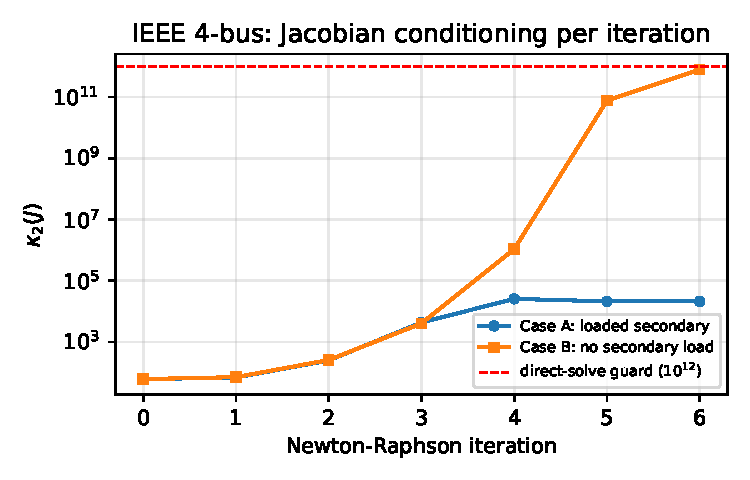
\includegraphics[width=\columnwidth]{fig1_4bus_conditioning}
\caption{IEEE 4-bus Jacobian conditioning per NR iteration. Case B (no
load on the Delta secondary) approaches the direct-solve guard threshold;
Case A (loaded secondary) stays four orders of magnitude below it.}
\label{fig:fourbus}
\end{figure}

\subsection{IEEE 13-bus: a doubly-floating network and solver oscillation}
\label{sec:results13}
The base paper's modification to the 13-node feeder --- reconnecting the
substation transformer T1 as Yg--Delta and the service transformer T2 as
Delta--Delta, with no other ground path anywhere in the reconstruction ---
leaves the network in a substantially more extreme regime than the 4-bus
case: the flat-start Jacobian is singular to machine precision
($\kappa_2 = 4.48\times10^{18}$) with \emph{exactly two} near-zero
singular values, not one. This matches a structural prediction: T1's
floating secondary leaves a common-mode direction spanning the entire
downstream network (everything except the source bus), while T2's
Delta--Delta connection additionally, and independently, floats bus 634
alone --- a Delta--Delta transformer's stamped zero-sequence transfer
block is exactly zero (Section~\ref{sec:background}), so the two floating
references are linearly independent.

At this feeder's corrected (post-bugfix, realistic) load level, the direct
solver fails everywhere by construction, and --- unexpectedly ---
\emph{so do SVD and RRQR}, once load exceeds roughly half of nominal
(Fig.~\ref{fig:robustness}). Both methods' undamped, exact minimum-norm
Newton steps oscillate rather than converge: $\|F\|_\infty$ fails to
decrease monotonically across iterations even after 80 iterations. Only
Tikhonov regularization ($\alpha = 10^{-8}$) converges cleanly at nominal
load, and it too eventually fails once load reaches $1.5\times$ nominal.
This is, to our knowledge, not a result the base paper's single-method
comparison could have surfaced: on this specific feeder, damping the
Newton step is not merely a way to handle exact singularity, but is
necessary for convergence \emph{at all} at realistic load.

\begin{figure}[t]
\centering
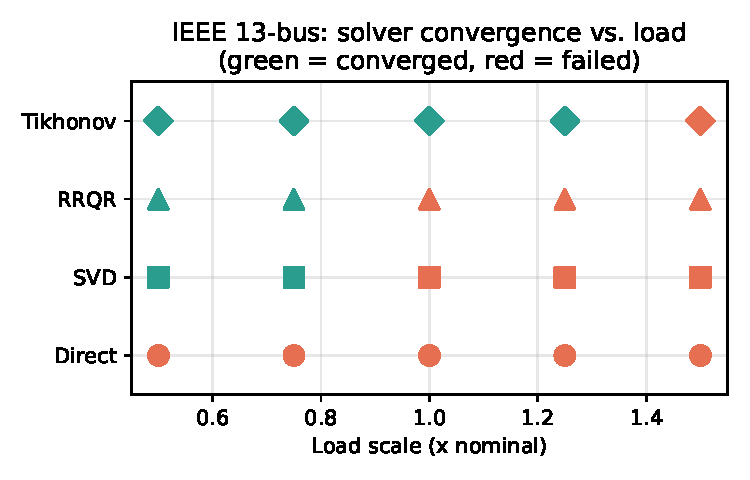
\includegraphics[width=\columnwidth]{fig2_ieee13_solver_robustness}
\caption{IEEE 13-bus solver convergence across a load-scaling sweep.
Direct always fails (the Jacobian is exactly singular by construction);
SVD and RRQR fail above $\sim0.75\times$ nominal load; only Tikhonov
converges through $1.25\times$, and even it fails at $1.5\times$.}
\label{fig:robustness}
\end{figure}

\subsection{Zero-sequence concentration under load imbalance}
\label{sec:zeroseq}
Using the symmetrical-component decomposition (Eq.~\eqref{eq:fortescue}),
we swept load imbalance from 0\% to 30\% (an explicitly documented,
non-paper-specified rule --- see Section~\ref{sec:limitations}) and
tracked the mean zero- and positive-sequence voltage magnitude across all
fully-three-phase buses. Zero-sequence magnitude $|V_0|$ grows
monotonically from 0.337 to 0.408\,pu (a 21\% relative increase) across
the sweep, while positive-sequence magnitude $|V_1|$ moves by under 1\%
(0.807 to 0.800\,pu; Fig.~\ref{fig:zeroseq}). Because $V_1$ is precisely
the physically meaningful, balanced component of voltage, this is a
direct, quantitative demonstration that load imbalance on a floating
network loads almost entirely onto the undetermined common-mode
component rather than the well-determined one --- a partial, structural
explanation for why a feeder with this topology (floating, unbalanced)
would show an outsized error relative to a better-grounded case, even
though the underlying network equations are solved to the same numerical
tolerance in both cases.

\begin{figure}[t]
\centering
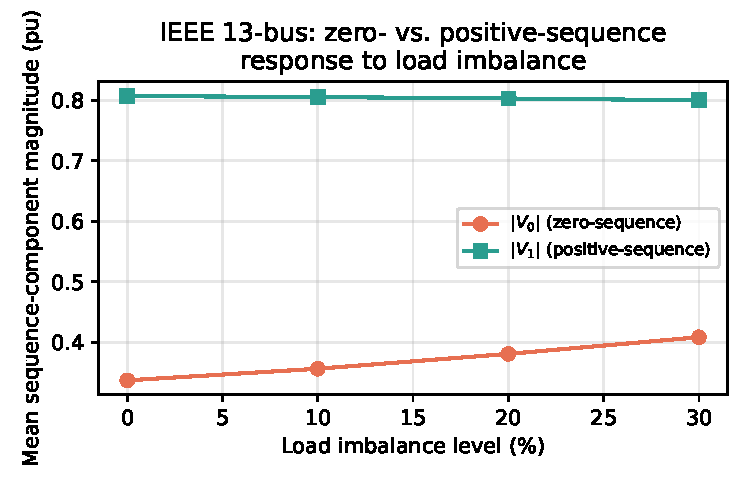
\includegraphics[width=\columnwidth]{fig3_ieee13_zero_sequence}
\caption{IEEE 13-bus: mean zero-sequence ($V_0$) and positive-sequence
($V_1$) voltage magnitude across a 0--30\% load-imbalance sweep. Nearly
all of the imbalance response loads onto $V_0$.}
\label{fig:zeroseq}
\end{figure}

Grounding both floating transformers (replacing their Delta windings with
grounded wye) confirms the causal story directly: $\kappa_2$ at flat start
falls from $4.48\times10^{18}$ to $773$ and mean $|V_0|$ falls from $0.337$
to $0.066$\,pu (Fig.~\ref{fig:grounding}). Grounding only one transformer
produces an intermediate result, isolating each transformer's independent
contribution to both the rank deficiency and the zero-sequence magnitude.

\begin{figure}[t]
\centering
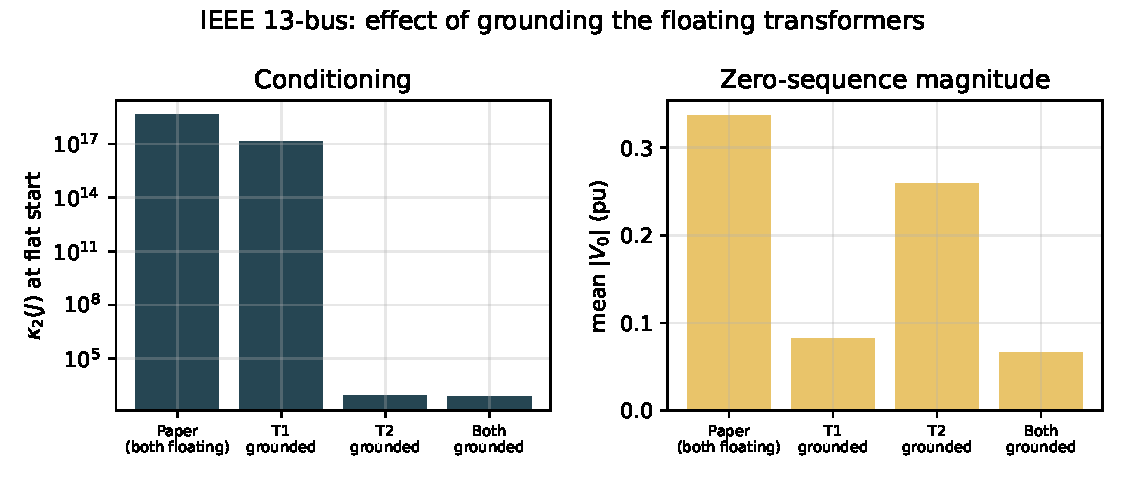
\includegraphics[width=\columnwidth]{fig4_ieee13_grounding}
\caption{IEEE 13-bus: progressively grounding T1 and/or T2 removes both
the extreme conditioning and the zero-sequence voltage magnitude,
isolating each transformer's independent contribution.}
\label{fig:grounding}
\end{figure}

\subsection{IEEE 37-bus: the reversal}
\label{sec:results37}
The IEEE 37-node feeder is, in its \emph{official, unmodified} form,
already close to the base paper's target configuration: both its
substation and service transformers are natively Delta--Delta, and the
service transformer's secondary already carries no load. The flat-start
Jacobian is again singular to machine precision
($\kappa_2 = 1.23\times10^{18}$), now with \emph{four} near-zero singular
values rather than two --- a larger, empirically-observed count we could
not fully derive analytically (an unloaded leaf bus behind one transformer
appears to contribute more than a single common-mode direction; see the
project repository's test suite for the full numerical investigation).

Despite the more extreme raw singular-value count, SVD and RRQR converge
\emph{cleanly} at nominal load here (10 iterations, no oscillation), while
Tikhonov regularization at the identical $\alpha = 10^{-8}$ used
successfully on the 13-bus feeder \emph{fails to converge} within 80
iterations on this feeder. This is the direct reversal of
Section~\ref{sec:results13}'s finding, and it is the paper's central
empirical result: \textbf{no single solver, and no single fixed
regularization strength, is uniformly best across feeder topologies.} The
practical difference between the two feeders is not the severity of the
worst-case singular value, but how much of the network a floating
transformer's secondary actually reaches: on the 13-bus feeder, T1's
floating region is essentially the entire downstream network; on the
37-bus feeder, the loads and topology are structured such that SVD/RRQR's
undamped step remains well-behaved even though the Jacobian is, by the
same $\kappa_2$ metric, comparably extreme.

Adding the paper's three quasi-radial loop-closing lines
(Section~\ref{sec:feeders}) changes $\kappa_2$ at flat start
($6.85\times10^{18}$, roughly $5.5\times$ larger) but not the qualitative
convergence picture: SVD still converges cleanly, and the count of
near-zero singular values (four) is unchanged, since the added loops do
not introduce a new floating region.

\subsection{IEEE 69-bus: severe conditioning without exact singularity}
\label{sec:results69}
The PG\&E 69-bus feeder, modified with three added Yg--Delta transformers
per the base paper's table, behaves differently again: the direct solver
\emph{converges} here ($\kappa_2 = 2.28\times10^5$ at flat start, growing to
$5.7\times10^{10}$ during iteration --- severe, but remaining under the
$10^{12}$ guard threshold). No singular value at flat start falls below
$10^{-6}\sigma_{\max}$ (smallest observed: $0.143$, against
$\sigma_{\max} = 3.26\times10^4$).

We verified numerically that $Y_{\mathrm{bus}}$ itself still has an exact
null direction across each transformer's floating downstream region (a
uniform complex voltage shift across the 47-bus region behind one
transformer leaves every branch current exactly unchanged, to within
$10^{-13}$). The reason the \emph{nonlinear} NR Jacobian does not inherit
this exact degeneracy is that the linearized mismatch in that direction is
proportional to the real current already flowing there at the operating
point, which is substantial on this feeder since the floating region
carries most of its real load. This is a genuine structural difference
from the 13- and 37-bus feeders, not a reconstruction artifact: whether a
floating-Delta topology produces an exactly singular flat-start Jacobian
depends on where the load sits relative to the floating region, not only
on the topology itself.

Because there is no exact null-space ambiguity on this feeder, its
OpenDSS cross-validation is essentially exact (median relative
line-to-line voltage error $3.3\times10^{-8}$, maximum $8.2\times10^{-6}$
--- Fig.~\ref{fig:crossval}), a useful negative control confirming that
the larger discrepancies on the 13- and 37-bus feeders
(Section~\ref{sec:crossval}) really do come from a genuinely
underdetermined subspace with more than one legitimate answer, not from a
limitation of either solver on the well-determined part of the problem.

\subsection{Cross-validation summary}
\label{sec:crossval}
Fig.~\ref{fig:crossval} summarizes the OpenDSS cross-validation error
across all reconstructions. The 13- and 37-bus feeders show median errors
of a few percent and maxima of several tens of percent, concentrated (by
construction) at the bus/phase pairs most aligned with each feeder's
near-null subspace; different regularizations --- this project's Tikhonov
solver versus OpenDSS's own internal \texttt{PPM\_Antifloat} regularization
--- select different particular solutions within that genuinely
underdetermined subspace, which is an expected consequence of the
singularity under study, not a validation failure. The 4- and 69-bus
feeders, which have no such exact ambiguity, agree with OpenDSS to
machine-precision-adjacent tolerances, providing exactly the negative
control that supports this reading.

\begin{figure}[t]
\centering
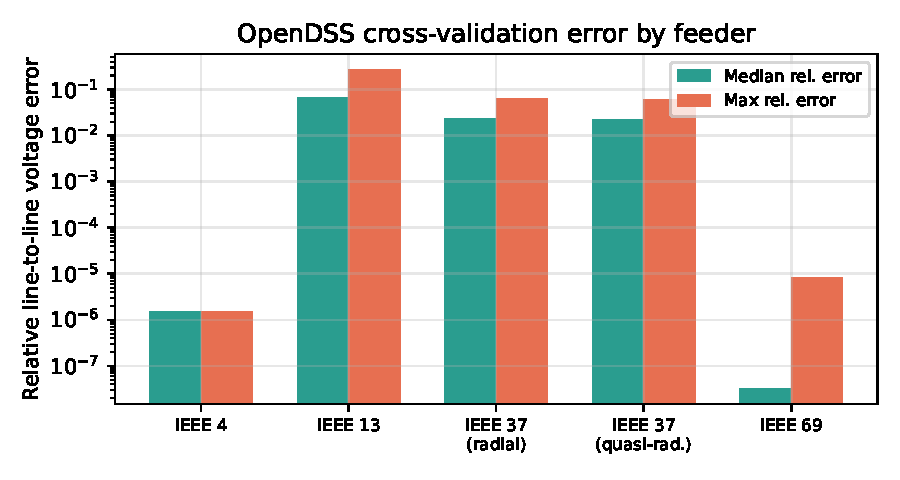
\includegraphics[width=\columnwidth]{fig6_crossvalidation_summary}
\caption{OpenDSS cross-validation error by feeder. The two feeders with an
exact null-space ambiguity (13, 37) show genuine disagreement in their
underdetermined subspace; the two without one (4, 69) agree to near
machine precision, a negative control supporting that reading.}
\label{fig:crossval}
\end{figure}

\subsection{IEEE 118-bus: linear-solver runtime scaling}
Following the base paper's use of a larger system purely for computational
scaling (not as further evidence about the singularity phenomenon), we
benchmarked all four solvers' wall-clock runtime on the real, converged
admittance matrix of \texttt{pandapower}'s \texttt{case118}
system~\cite{thurner2018pandapower}, block-diagonally replicated up to
$8\times$ to obtain a scaling curve from a genuine (not synthetic random)
sparse structure at each size (Fig.~\ref{fig:scaling}). All four solvers
show empirical wall-clock scaling exponents between 2.15 and 2.39 across
matrix sizes from 236 to 1888 (real-valued Jacobian form), sub-cubic at
these sizes as expected from BLAS-level dense-solver optimization rather
than the na\"ive $O(n^3)$ asymptotic bound. Tikhonov is consistently the
slowest of the four (its augmented system has $50\%$ more rows than the
others' $n \times n$ systems), and direct is consistently the fastest,
though the relative overhead of SVD/RRQR/Tikhonov over direct narrows only
slightly across this size range.

\begin{figure}[t]
\centering
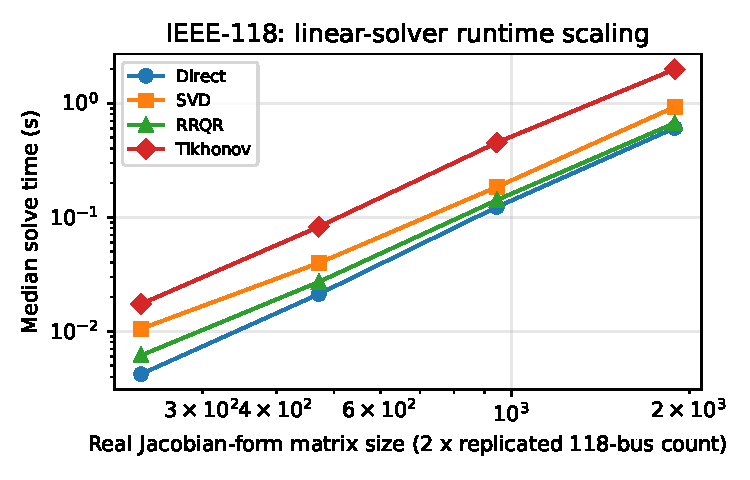
\includegraphics[width=\columnwidth]{fig5_ieee118_scaling}
\caption{Linear-solver runtime scaling on the real (replicated)
IEEE-118 admittance matrix, log-log.}
\label{fig:scaling}
\end{figure}

\section{Discussion}
\label{sec:discussion}

The central methodological claim of this paper is that \textbf{solver
choice for a singular or ill-conditioned NR Jacobian should be matched to
the structure of the rank deficiency, not chosen once and applied
uniformly}. The base paper's Moore--Penrose pseudo-inverse is a principled
and effective choice when the floating region is small relative to the
rest of the network (as on the 69-bus feeder, where it is not even
strictly necessary) or when the network's overall behavior tolerates an
undamped exact-minimum-norm step (as on the 37-bus feeder). But on the
13-bus feeder, where the paper-specified modification floats essentially
the entire downstream network, that same undamped step oscillates at
realistic load, and only an explicitly damped, regularized step
(Tikhonov) converges at all. Neither SVD nor RRQR is "wrong" in any
absolute sense on the 13-bus feeder --- both correctly compute the
minimum-norm solution to their respective linearized sub-problems at every
iteration --- but the sequence of such steps fails to make global
progress on the underlying nonlinear problem. This is a genuinely
different failure mode from the exact-singularity failure the base paper
addresses, and RRQR (despite being algebraically closely related to SVD:
both compute an exact minimum-norm least-squares solution for the
linearized step) inherits the same oscillation, which rules out "RRQR
instead of SVD" as a fix on its own.

This reframes the base paper's open question about the 13-bus feeder's
elevated error. Our zero-sequence investigation (Section~\ref{sec:zeroseq})
shows that load imbalance on this specific feeder's topology loads almost
entirely onto the zero-sequence component, which is precisely the
component a floating Delta-connected transformer leaves undetermined. A
solver that reports a converged, low-residual solution is not thereby
reporting a \emph{unique} solution when the underlying linear system is
rank-deficient; different, individually defensible regularization choices
(this project's Tikhonov solver, OpenDSS's internal
\texttt{PPM\_Antifloat} admittance) will disagree specifically in that
undetermined direction, and the base paper's reported error, computed
against a single reference solver, may in part be measuring exactly this
ambiguity rather than a shortcoming of the Moore--Penrose approach itself.
We do not claim this fully explains the base paper's reported
$2.08\times10^{-4}$\,pu figure --- our reconstruction is independent of
theirs and not intended as an exact reproduction (Section~\ref{sec:limitations})
--- but the mechanism we demonstrate here (imbalance concentrating in
$V_0$ on a floating network) is a directly testable, structural candidate
explanation that the base paper's single-solver, single-feeder-instance
comparison could not have isolated on its own.

\section{Limitations and Open Discrepancies}
\label{sec:limitations}

Consistent with this project's policy of documenting rather than silently
resolving ambiguity in the base paper or the official source data, the
following remain open:

\begin{itemize}
\item \textbf{IEEE 13-bus load count.} The base paper states its modified
13-bus case has seven loads. After removing the one location its own
description unambiguously identifies (the distributed-load stand-in on
line 632--671), the official feeder data still has \emph{eight} distinct
load locations, not seven. Rather than arbitrarily delete one further real
load to force a numeric match, our reconstruction keeps all eight.
\item \textbf{IEEE 37-bus XFM1 reactance.} The base paper reports
$X \approx 0.00181$\,pu for the service transformer; the official OpenDSS
model gives $X_{hl} = 1.81\%$ (i.e., $0.0181$\,pu on the transformer's own
base) --- an apparent factor-of-ten discrepancy. Our reconstruction uses
the officially-sourced value by default and exposes the alternate reading
as a parameter, without asserting which is correct.
\item \textbf{IEEE 69-bus voltage base.} The base paper's added-transformer
table specifies 13.8\,kV; the underlying MATPOWER \texttt{case69} network
operates at 12.66\,kV. We use the network's actual operating voltage and
flag the mismatch rather than silently reconciling it.
\item \textbf{Delta-connected loads.} All three larger feeders contain
delta-connected loads (a single leg or a full three-phase delta object).
Because the shared mismatch model supports only phase-to-neutral
constant-PQ injection, every delta load is approximated as an even
wye-equivalent split across its connected phases --- a standard simplified
load-flow approximation, not an attempt to reproduce delta-branch current
physics exactly.
\item \textbf{Voltage regulators.} Discrete tap-changing voltage regulators
present in the official 13- and 37-bus feeders are modeled as ideal
(zero-impedance, fixed-ratio) connections. Modeling their discrete control
logic is a materially different (hybrid discrete/continuous) numerical
problem, out of scope for a study of the underlying linear-solver
comparison.
\item \textbf{Load-imbalance construction.} Neither the base paper nor the
official feeder data specify a phase-by-phase rule for constructing an
imbalanced load case. Our imbalance sweep (Section~\ref{sec:zeroseq}) uses
an explicitly documented, project-defined rule (scaling phase~a's load by
$1+L$ and phase~c's by $1-L$ at imbalance level $L$), chosen for its
monotonic, roughly load-neutral behavior rather than as a claim about the
base paper's own (undocumented) construction.
\end{itemize}

We regard this list as a strength of the reconstruction methodology rather
than a weakness: every entry reflects a place where the source material
itself is ambiguous or incomplete, made explicit rather than resolved by
assumption.

\section{Conclusion}
\label{sec:conclusion}

We built a shared three-phase Newton--Raphson engine and compared direct,
SVD/Moore--Penrose, rank-revealing QR, and Tikhonov-regularized linear
solves across four independently reconstructed and cross-validated IEEE/PG\&E
test feeders. The central result is that no single method dominates: the
same undamped, exact minimum-norm step that the base paper's pseudo-inverse
approach relies on oscillates rather than converges on a feeder whose
floating transformer secondary spans the entire downstream network (IEEE
13-bus) at realistic load, while the identical Tikhonov regularization that
rescues that case fails outright on a feeder where SVD and RRQR converge
cleanly (IEEE 37-bus). A controlled symmetrical-component investigation
shows that load imbalance on the 13-bus feeder's topology concentrates
almost entirely in the zero-sequence voltage component, offering a
structural, partially explanatory account of that feeder's characteristic
elevated error. Finally, this project's own development process
demonstrates the practical value of independent cross-validation: two real,
independent per-unit modeling bugs were caught only by validating
small, well-conditioned sub-circuits against an external solver before
trusting comparisons on the full, already-ill-conditioned systems --- a
discipline we recommend as a matter of course for any project reconstructing
power-system test cases from published, and inevitably sometimes
under-specified, sources.

\section*{Acknowledgment}
This work reproduces and extends the numerical methodology of Jang,
Kim, and Kim~\cite{jang2023singularity}. Test feeder data are drawn from
the IEEE PES Distribution System Analysis Subcommittee's public test
feeder repository~\cite{ieeetestfeeders} and the MATPOWER
project~\cite{zimmerman2011matpower}, originally from Baran and
Wu~\cite{baran1989network}. Independent validation used
OpenDSS~\cite{opendss} and pandapower~\cite{thurner2018pandapower}.

\bibliographystyle{IEEEtran}
\bibliography{refs}

\end{document}